{}

\section{{Problem 1}}

	\subsection{{Computer Program}}

		\begin{lstlisting}[language=C, caption=\textit{}]
#include <stdio.h>

void main(void)
{
    FILE* file;
    int amt, i;
    double min, max, x1, xh;
    file = fopen("data.txt", "r");
    while (!feof(file))
    {
        fscanf(file, "%d %lf %lf", &amt, &min, &max);
        double nums[amt], norm[amt];
        for (int i = 0; i < amt; i++)
        {
            fscanf(file, "%lf", &nums[i]);
        }
        x1 = nums[0];
        xh = nums[1];
        for (int i = 0; i < amt; i++)
        {
            if (nums[i] < x1)
            {
                x1 = nums[i];
            }
            else if (nums[i] > xh)
            {
                xh = nums[i];
            }            
        }
        for (int i = 0; i < amt; i++)
        {
            norm[i] = min + ((nums[i] - xh) * (max - min) / (xh - x1));
        }
        printf("Original\t\tNormalized\n");
        printf("--------    ----------\n");
        for (int i = 0; i < amt; i++)
        {
            printf("%.1lf\t\t%.1lf\n", nums[i], norm[i]);
        }
        fclose(file);
    }
}


\end{lstlisting}

	\subsection{{Program Output Screenshot}}

		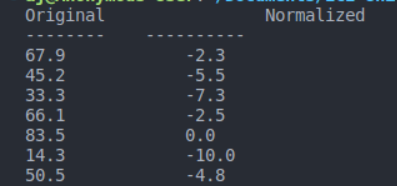
\includegraphics[width=15cm]{problem1.png}
		
\section{{Problem 2}}
	
		\subsection{{Computer Program}}
	
			\begin{lstlisting}[language=C, caption=\textit{}]	


#include <stdio.h>
#define ARRAY_SIZE 8
//  finds the position of the smallest element in the subarray
//  list[first] through list[last].
//  Pre: first < last and elements 0 through last of array list are defined.
//  Post: Returns the subscript k of the smallest element in the subarray;
//  i.e., list[k] <= list[i] for all i in the subarray
int get_min_range (int list[], int first, int last)
{
    int j;
    int min = sizeof(double);
    for (int i = 0; i < last; i++)
    {
        if (min > list[i])
        {
            min = list[i];
            j = i;
        }
    }
    return j;
}
//  sorts the data in array list
void select_sort(int list[], int n)
{
    int fill,   /*  index of first element in unsorted subarray */
    temp,   /*  temporary storage   */
    index_of_min;   /*  subscript of next smallest element  */
    for (fill = 0; fill < n-1; ++fill)
    {
        /*  Find position of smallest element in unsorted subarray */
        index_of_min = get_min_range (list, fill, n-1);
        /* Exchange elements at fill and index_of_min */
        if (fill != index_of_min)
        {
            temp = list[index_of_min];
            list[index_of_min] = list[fill];
            list[fill] = temp;
        }
    }
}
int main (void)
{
    int array[] = {67, 98, 23, 11, 47, 13, 94, 58};
    int i;
    select_sort (array, ARRAY_SIZE);
    for (i=0; i < 8; ++i)
    {
        printf ("%d ", array[i]);
    } printf("\n");
    return (0);
}

	\end{lstlisting}

		\subsection{{Program Output Screenshot}}
			
			{}
			
			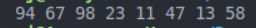
\includegraphics[width=12.75cm]{problem2.png}


\section{{Problem 3}}
	
	\subsection{{Computer Program}}
	
		\begin{lstlisting}[language=C, caption=\textit{}]	
#include <stdio.h>
#define STACK_EMPTY '0'
#define STACK_SIZE 20

void push(char stack[], /* input/output - the stack */
char item, /* input - data being pushed onto the stack */
int *top, /* input/output - pointer to top of stack */
int max_size) /* input - maximum size of stack */
{
    if (*top < max_size-1)
    {
        ++(*top);
        stack[*top] = item;
    }
}
char pop (char stack[], /* input/output - the stack */
int *top) /* input/output - pointer to top of stack */
{
    char item; /* value popped off the stack */
    if (*top >= 0)
    {
        item = stack[*top];
        --(*top);
    }
    else
    {
        item = STACK_EMPTY;
    }
    return (item);
}
void main(void)
{
    char s [STACK_SIZE];
    int s_top = -1; // stack is empty
    int *ptr = &s_top;
    push(s, 'A', ptr, STACK_SIZE);
    push(s, 'B', ptr, STACK_SIZE);
    push(s, 'C', ptr, STACK_SIZE);

    for (int i = 0; i < *ptr; i++)
    {
        printf("%c", s[i]);
    }
    printf("\n");
    pop(s, ptr);
    for (int i = 0; i < *ptr; i++)
    {
        printf("%c", s[i]);
    }
}

	\end{lstlisting}
	
	\subsection{{Program Output Screenshot}}
	
		{}
		
		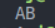
\includegraphics[width=12.75cm]{problem3.png}
		
		
		